\chapter{Sortierverfahren}
\renewcommand{\chaptertitle}{Sortierverfahren}

\lehead[]{\sf\hspace*{-2.00cm}\textcolor{white}{\colorbox{lightblue}{\makebox[1.60cm][r]{\thechapter}}}\hspace{0.17cm}\textcolor{lightblue}{\chaptertitle}}
\rohead[]{\textcolor{lightblue}{\chaptertitle}\sf\hspace*{0.17cm}\textcolor{white}{\colorbox{lightblue}{\makebox[1.60cm][l]{\thechapter}}}\hspace{-2.00cm}}
%\chead[]{}
\rehead[]{\textcolor{lightblue}{AvHG, Inf, My}}
\lohead[]{\textcolor{lightblue}{AvHG, Inf, My}}

\lstset{style=myJava}

Dieses Thema soll zunächst in Gruppen erarbeitet werden. Dazu wird die Klasse in
drei etwa gleich große Gruppen eingeteilt. Jede Gruppe erhält ein anderes
Sortierverfahren und soll dieses Verfahren verstehen. Anschließend sollen die
Gruppenmitglieder vier Zahlen mit ihrem Verfahren sortieren.

Zum Ausprobieren bekommt jede Gruppe ein Kartenset!

Jede Gruppe beschreibt ihr Sortierverfahren schriftlich (Die Beschreibungen
werden am Schluss der Übung für alle ausgedruckt). Außerdem sollen sie einen
Vortrag über ihr Sortierverfahren für die anderen Schüler vorbereiten.

Die folgenden zwei Aufgaben sollen von jeder der drei Gruppen bearbeitet werden:

\begin{compactenum}[a)]
\item Erklärt das Sortierverfahren.
\item Sortiert mit euren Regeln die Zahlenreihe „8 3 1 7“. Schreibt dabei die Zahlenreihe nach jedem Schritt auf.
\end{compactenum}

Nach den Gruppen-Vorträgen sollen die Übungen in Einzelarbeit gelöst werden.

\clearpage

\section{Gruppe 1: Sortieren durch Einfügen (Insertion Sort)}

Nach welchen Regeln werden die Karten sortiert?

Tipp: Gehe von unten nach oben. Markiere die Kartenmenge, die sortiert ist. Der
sortierte Teil wird von oben her immer größer.

\begin{tabular}{m{30mm}m{11mm}m{11mm}m{11mm}m{11mm}m{11mm}m{11mm}m{11mm}m{11mm}}
Ausgangssituation: &
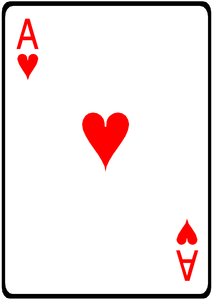
\includegraphics[width=0.08\textwidth]{./inf/SEKII/19_Java_Sortierverfahren/HerzAs.png}
&
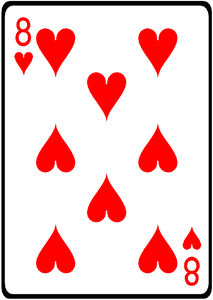
\includegraphics[width=0.08\textwidth]{./inf/SEKII/19_Java_Sortierverfahren/Herz8.png}
&
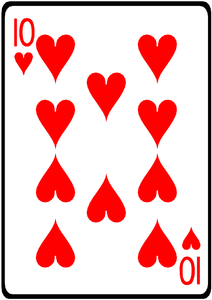
\includegraphics[width=0.08\textwidth]{./inf/SEKII/19_Java_Sortierverfahren/Herz10.png}
&
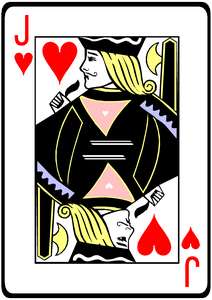
\includegraphics[width=0.08\textwidth]{./inf/SEKII/19_Java_Sortierverfahren/HerzBube.png}
&
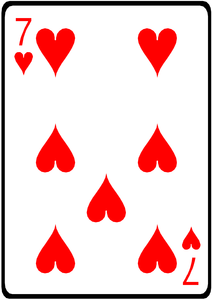
\includegraphics[width=0.08\textwidth]{./inf/SEKII/19_Java_Sortierverfahren/Herz7.png}
&
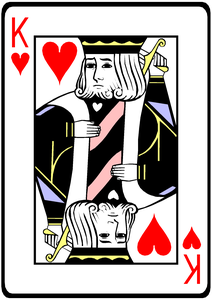
\includegraphics[width=0.08\textwidth]{./inf/SEKII/19_Java_Sortierverfahren/HerzKoenig.png}
&
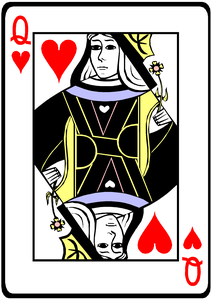
\includegraphics[width=0.08\textwidth]{./inf/SEKII/19_Java_Sortierverfahren/HerzDame.png}
&
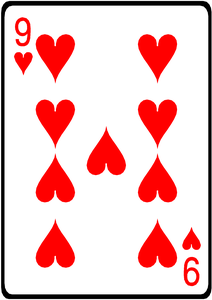
\includegraphics[width=0.08\textwidth]{./inf/SEKII/19_Java_Sortierverfahren/Herz9.png}
\\
Nach dem 1.\ Schritt: &
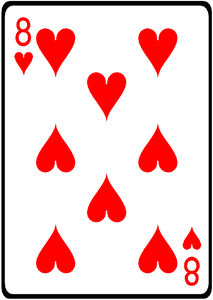
\includegraphics[width=0.08\textwidth]{./inf/SEKII/19_Java_Sortierverfahren/Herz8.png}
&
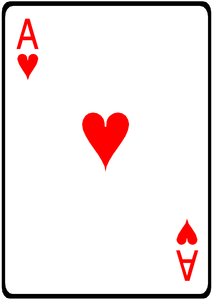
\includegraphics[width=0.08\textwidth]{./inf/SEKII/19_Java_Sortierverfahren/HerzAs.png}
&
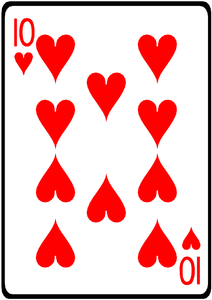
\includegraphics[width=0.08\textwidth]{./inf/SEKII/19_Java_Sortierverfahren/Herz10.png}
&
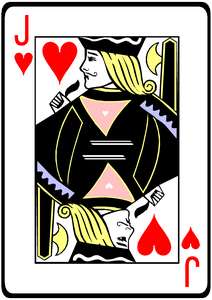
\includegraphics[width=0.08\textwidth]{./inf/SEKII/19_Java_Sortierverfahren/HerzBube.png}
&
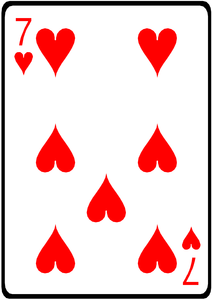
\includegraphics[width=0.08\textwidth]{./inf/SEKII/19_Java_Sortierverfahren/Herz7.png}
&
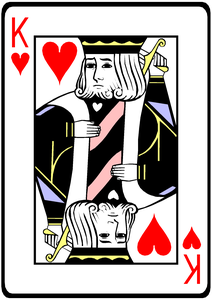
\includegraphics[width=0.08\textwidth]{./inf/SEKII/19_Java_Sortierverfahren/HerzKoenig.png}
&
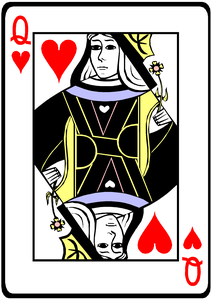
\includegraphics[width=0.08\textwidth]{./inf/SEKII/19_Java_Sortierverfahren/HerzDame.png}
&
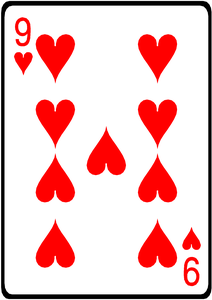
\includegraphics[width=0.08\textwidth]{./inf/SEKII/19_Java_Sortierverfahren/Herz9.png}
\\
Nach dem 2.\ Schritt: &
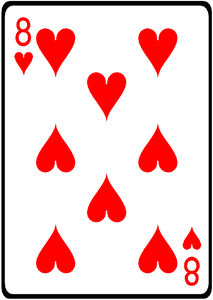
\includegraphics[width=0.08\textwidth]{./inf/SEKII/19_Java_Sortierverfahren/Herz8.png}
&
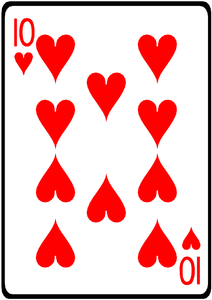
\includegraphics[width=0.08\textwidth]{./inf/SEKII/19_Java_Sortierverfahren/Herz10.png}
&
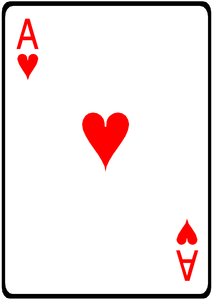
\includegraphics[width=0.08\textwidth]{./inf/SEKII/19_Java_Sortierverfahren/HerzAs.png}
&
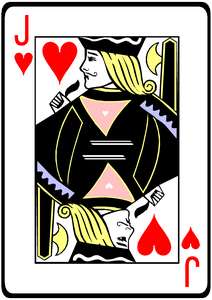
\includegraphics[width=0.08\textwidth]{./inf/SEKII/19_Java_Sortierverfahren/HerzBube.png}
&
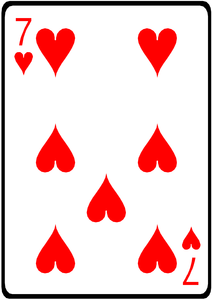
\includegraphics[width=0.08\textwidth]{./inf/SEKII/19_Java_Sortierverfahren/Herz7.png}
&
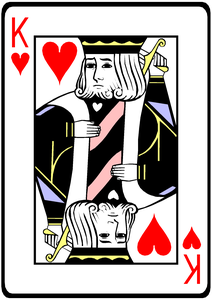
\includegraphics[width=0.08\textwidth]{./inf/SEKII/19_Java_Sortierverfahren/HerzKoenig.png}
&
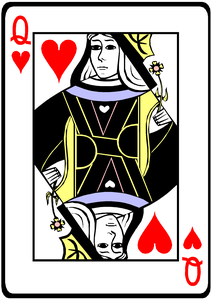
\includegraphics[width=0.08\textwidth]{./inf/SEKII/19_Java_Sortierverfahren/HerzDame.png}
&
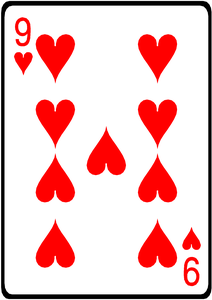
\includegraphics[width=0.08\textwidth]{./inf/SEKII/19_Java_Sortierverfahren/Herz9.png}
\\
Nach dem 3.\ Schritt: &
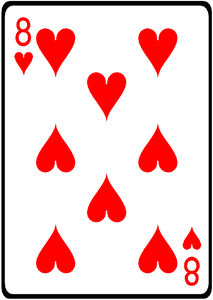
\includegraphics[width=0.08\textwidth]{./inf/SEKII/19_Java_Sortierverfahren/Herz8.png}
&
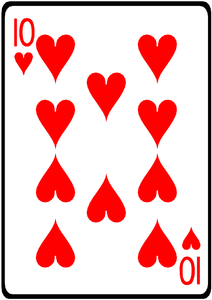
\includegraphics[width=0.08\textwidth]{./inf/SEKII/19_Java_Sortierverfahren/Herz10.png}
&
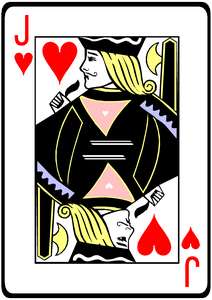
\includegraphics[width=0.08\textwidth]{./inf/SEKII/19_Java_Sortierverfahren/HerzBube.png}
&
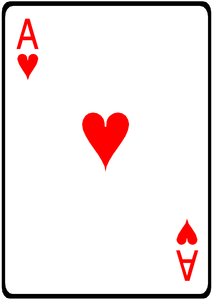
\includegraphics[width=0.08\textwidth]{./inf/SEKII/19_Java_Sortierverfahren/HerzAs.png}
&
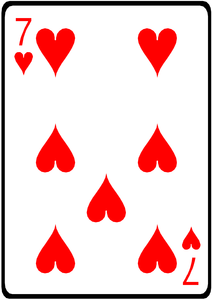
\includegraphics[width=0.08\textwidth]{./inf/SEKII/19_Java_Sortierverfahren/Herz7.png}
&
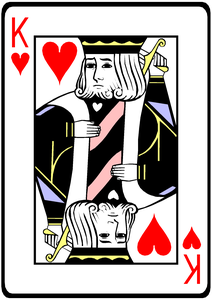
\includegraphics[width=0.08\textwidth]{./inf/SEKII/19_Java_Sortierverfahren/HerzKoenig.png}
&
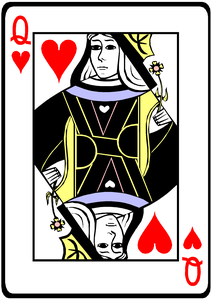
\includegraphics[width=0.08\textwidth]{./inf/SEKII/19_Java_Sortierverfahren/HerzDame.png}
&
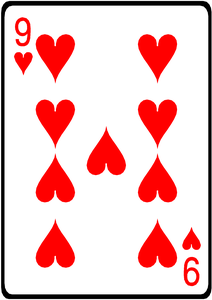
\includegraphics[width=0.08\textwidth]{./inf/SEKII/19_Java_Sortierverfahren/Herz9.png}
\\
Nach dem 4.\ Schritt: &
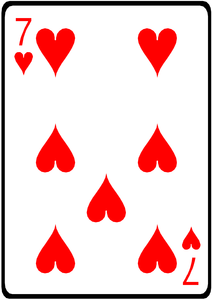
\includegraphics[width=0.08\textwidth]{./inf/SEKII/19_Java_Sortierverfahren/Herz7.png}
&
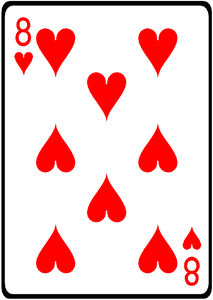
\includegraphics[width=0.08\textwidth]{./inf/SEKII/19_Java_Sortierverfahren/Herz8.png}
&
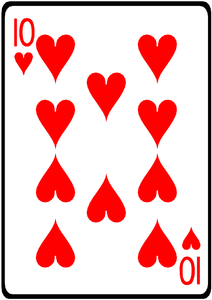
\includegraphics[width=0.08\textwidth]{./inf/SEKII/19_Java_Sortierverfahren/Herz10.png}
&
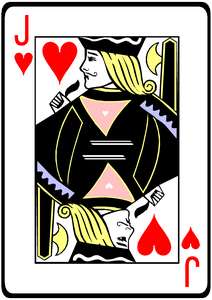
\includegraphics[width=0.08\textwidth]{./inf/SEKII/19_Java_Sortierverfahren/HerzBube.png}
&
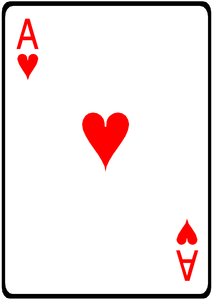
\includegraphics[width=0.08\textwidth]{./inf/SEKII/19_Java_Sortierverfahren/HerzAs.png}
&
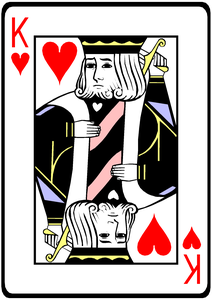
\includegraphics[width=0.08\textwidth]{./inf/SEKII/19_Java_Sortierverfahren/HerzKoenig.png}
&
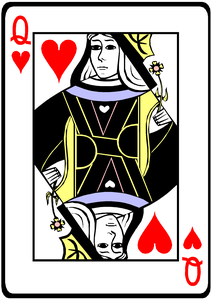
\includegraphics[width=0.08\textwidth]{./inf/SEKII/19_Java_Sortierverfahren/HerzDame.png}
&
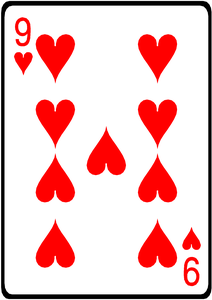
\includegraphics[width=0.08\textwidth]{./inf/SEKII/19_Java_Sortierverfahren/Herz9.png}
\\
Nach dem 5.\ Schritt: &
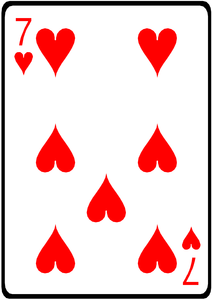
\includegraphics[width=0.08\textwidth]{./inf/SEKII/19_Java_Sortierverfahren/Herz7.png}
&
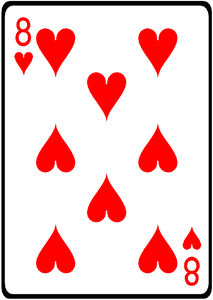
\includegraphics[width=0.08\textwidth]{./inf/SEKII/19_Java_Sortierverfahren/Herz8.png}
&
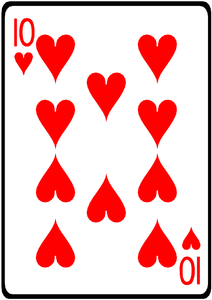
\includegraphics[width=0.08\textwidth]{./inf/SEKII/19_Java_Sortierverfahren/Herz10.png}
&
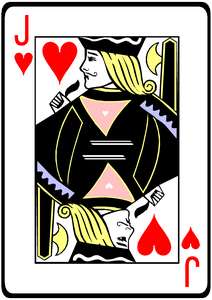
\includegraphics[width=0.08\textwidth]{./inf/SEKII/19_Java_Sortierverfahren/HerzBube.png}
&
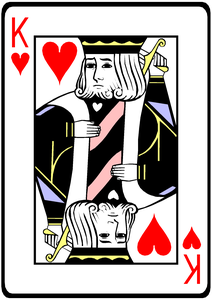
\includegraphics[width=0.08\textwidth]{./inf/SEKII/19_Java_Sortierverfahren/HerzKoenig.png}
&
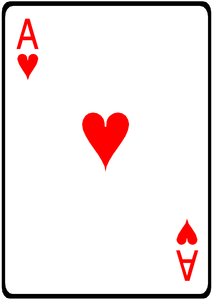
\includegraphics[width=0.08\textwidth]{./inf/SEKII/19_Java_Sortierverfahren/HerzAs.png}
&
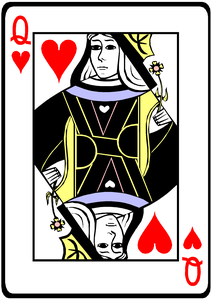
\includegraphics[width=0.08\textwidth]{./inf/SEKII/19_Java_Sortierverfahren/HerzDame.png}
&
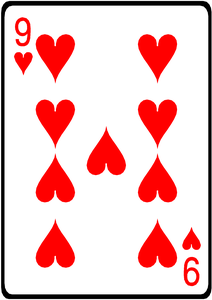
\includegraphics[width=0.08\textwidth]{./inf/SEKII/19_Java_Sortierverfahren/Herz9.png}
\\
Nach dem 6.\ Schritt: &
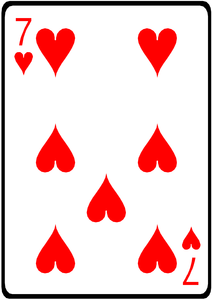
\includegraphics[width=0.08\textwidth]{./inf/SEKII/19_Java_Sortierverfahren/Herz7.png}
&
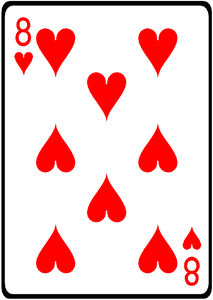
\includegraphics[width=0.08\textwidth]{./inf/SEKII/19_Java_Sortierverfahren/Herz8.png}
&
\includegraphics[width=0.08\textwidth]{./inf/SEKII/19_Java_Sortierverfahren/Herz10.png}
&
\includegraphics[width=0.08\textwidth]{./inf/SEKII/19_Java_Sortierverfahren/HerzBube.png}
&
\includegraphics[width=0.08\textwidth]{./inf/SEKII/19_Java_Sortierverfahren/HerzDame.png}
&
\includegraphics[width=0.08\textwidth]{./inf/SEKII/19_Java_Sortierverfahren/HerzKoenig.png}
&
\includegraphics[width=0.08\textwidth]{./inf/SEKII/19_Java_Sortierverfahren/HerzAs.png}
&
\includegraphics[width=0.08\textwidth]{./inf/SEKII/19_Java_Sortierverfahren/Herz9.png}
\\
Nach dem 7.\ Schritt: &
\includegraphics[width=0.08\textwidth]{./inf/SEKII/19_Java_Sortierverfahren/Herz7.png}
&
\includegraphics[width=0.08\textwidth]{./inf/SEKII/19_Java_Sortierverfahren/Herz8.png}
&
\includegraphics[width=0.08\textwidth]{./inf/SEKII/19_Java_Sortierverfahren/Herz9.png}
&
\includegraphics[width=0.08\textwidth]{./inf/SEKII/19_Java_Sortierverfahren/Herz10.png}
&
\includegraphics[width=0.08\textwidth]{./inf/SEKII/19_Java_Sortierverfahren/HerzBube.png}
&
\includegraphics[width=0.08\textwidth]{./inf/SEKII/19_Java_Sortierverfahren/HerzDame.png}
&
\includegraphics[width=0.08\textwidth]{./inf/SEKII/19_Java_Sortierverfahren/HerzKoenig.png}
&
\includegraphics[width=0.08\textwidth]{./inf/SEKII/19_Java_Sortierverfahren/HerzAs.png}
\\
\end{tabular}

\clearpage


\section{Gruppe 2: Sortieren durch Auswählen (Selection Sort)}

Nach welchen Regeln werden die Karten sortiert?

Tipp: Ab welchem Schritt steht die Karte an der richtigen Position?

\begin{tabular}{m{30mm}m{11mm}m{11mm}m{11mm}m{11mm}m{11mm}m{11mm}m{11mm}m{11mm}}
Ausgangssituation: &
\includegraphics[width=0.08\textwidth]{./inf/SEKII/19_Java_Sortierverfahren/KaroAs.png}
&
\includegraphics[width=0.08\textwidth]{./inf/SEKII/19_Java_Sortierverfahren/Karo8.png}
&
\includegraphics[width=0.08\textwidth]{./inf/SEKII/19_Java_Sortierverfahren/Karo10.png}
&
\includegraphics[width=0.08\textwidth]{./inf/SEKII/19_Java_Sortierverfahren/KaroBube.png}
&
\includegraphics[width=0.08\textwidth]{./inf/SEKII/19_Java_Sortierverfahren/Karo7.png}
&
\includegraphics[width=0.08\textwidth]{./inf/SEKII/19_Java_Sortierverfahren/KaroKoenig.png}
&
\includegraphics[width=0.08\textwidth]{./inf/SEKII/19_Java_Sortierverfahren/KaroDame.png}
&
\includegraphics[width=0.08\textwidth]{./inf/SEKII/19_Java_Sortierverfahren/Karo9.png}
\\
Nach dem 1.\ Schritt: &
\includegraphics[width=0.08\textwidth]{./inf/SEKII/19_Java_Sortierverfahren/Karo7.png}
&
\includegraphics[width=0.08\textwidth]{./inf/SEKII/19_Java_Sortierverfahren/Karo8.png}
&
\includegraphics[width=0.08\textwidth]{./inf/SEKII/19_Java_Sortierverfahren/Karo10.png}
&
\includegraphics[width=0.08\textwidth]{./inf/SEKII/19_Java_Sortierverfahren/KaroBube.png}
&
\includegraphics[width=0.08\textwidth]{./inf/SEKII/19_Java_Sortierverfahren/KaroAs.png}
&
\includegraphics[width=0.08\textwidth]{./inf/SEKII/19_Java_Sortierverfahren/KaroKoenig.png}
&
\includegraphics[width=0.08\textwidth]{./inf/SEKII/19_Java_Sortierverfahren/KaroDame.png}
&
\includegraphics[width=0.08\textwidth]{./inf/SEKII/19_Java_Sortierverfahren/Karo9.png}
\\
Nach dem 2.\ Schritt: &
\includegraphics[width=0.08\textwidth]{./inf/SEKII/19_Java_Sortierverfahren/Karo7.png}
&
\includegraphics[width=0.08\textwidth]{./inf/SEKII/19_Java_Sortierverfahren/Karo8.png}
&
\includegraphics[width=0.08\textwidth]{./inf/SEKII/19_Java_Sortierverfahren/Karo10.png}
&
\includegraphics[width=0.08\textwidth]{./inf/SEKII/19_Java_Sortierverfahren/KaroBube.png}
&
\includegraphics[width=0.08\textwidth]{./inf/SEKII/19_Java_Sortierverfahren/KaroAs.png}
&
\includegraphics[width=0.08\textwidth]{./inf/SEKII/19_Java_Sortierverfahren/KaroKoenig.png}
&
\includegraphics[width=0.08\textwidth]{./inf/SEKII/19_Java_Sortierverfahren/KaroDame.png}
&
\includegraphics[width=0.08\textwidth]{./inf/SEKII/19_Java_Sortierverfahren/Karo9.png}
\\
Nach dem 3.\ Schritt: &
\includegraphics[width=0.08\textwidth]{./inf/SEKII/19_Java_Sortierverfahren/Karo7.png}
&
\includegraphics[width=0.08\textwidth]{./inf/SEKII/19_Java_Sortierverfahren/Karo8.png}
&
\includegraphics[width=0.08\textwidth]{./inf/SEKII/19_Java_Sortierverfahren/Karo9.png}
&
\includegraphics[width=0.08\textwidth]{./inf/SEKII/19_Java_Sortierverfahren/KaroBube.png}
&
\includegraphics[width=0.08\textwidth]{./inf/SEKII/19_Java_Sortierverfahren/KaroAs.png}
&
\includegraphics[width=0.08\textwidth]{./inf/SEKII/19_Java_Sortierverfahren/KaroKoenig.png}
&
\includegraphics[width=0.08\textwidth]{./inf/SEKII/19_Java_Sortierverfahren/KaroDame.png}
&
\includegraphics[width=0.08\textwidth]{./inf/SEKII/19_Java_Sortierverfahren/Karo10.png}
\\
Nach dem 4.\ Schritt: &
\includegraphics[width=0.08\textwidth]{./inf/SEKII/19_Java_Sortierverfahren/Karo7.png}
&
\includegraphics[width=0.08\textwidth]{./inf/SEKII/19_Java_Sortierverfahren/Karo8.png}
&
\includegraphics[width=0.08\textwidth]{./inf/SEKII/19_Java_Sortierverfahren/Karo9.png}
&
\includegraphics[width=0.08\textwidth]{./inf/SEKII/19_Java_Sortierverfahren/Karo10.png}
&
\includegraphics[width=0.08\textwidth]{./inf/SEKII/19_Java_Sortierverfahren/KaroAs.png}
&
\includegraphics[width=0.08\textwidth]{./inf/SEKII/19_Java_Sortierverfahren/KaroKoenig.png}
&
\includegraphics[width=0.08\textwidth]{./inf/SEKII/19_Java_Sortierverfahren/KaroDame.png}
&
\includegraphics[width=0.08\textwidth]{./inf/SEKII/19_Java_Sortierverfahren/KaroBube.png}
\\
Nach dem 5.\ Schritt: &
\includegraphics[width=0.08\textwidth]{./inf/SEKII/19_Java_Sortierverfahren/Karo7.png}
&
\includegraphics[width=0.08\textwidth]{./inf/SEKII/19_Java_Sortierverfahren/Karo8.png}
&
\includegraphics[width=0.08\textwidth]{./inf/SEKII/19_Java_Sortierverfahren/Karo9.png}
&
\includegraphics[width=0.08\textwidth]{./inf/SEKII/19_Java_Sortierverfahren/Karo10.png}
&
\includegraphics[width=0.08\textwidth]{./inf/SEKII/19_Java_Sortierverfahren/KaroBube.png}
&
\includegraphics[width=0.08\textwidth]{./inf/SEKII/19_Java_Sortierverfahren/KaroKoenig.png}
&
\includegraphics[width=0.08\textwidth]{./inf/SEKII/19_Java_Sortierverfahren/KaroDame.png}
&
\includegraphics[width=0.08\textwidth]{./inf/SEKII/19_Java_Sortierverfahren/KaroAs.png}
\\
Nach dem 6.\ Schritt: &
\includegraphics[width=0.08\textwidth]{./inf/SEKII/19_Java_Sortierverfahren/Karo7.png}
&
\includegraphics[width=0.08\textwidth]{./inf/SEKII/19_Java_Sortierverfahren/Karo8.png}
&
\includegraphics[width=0.08\textwidth]{./inf/SEKII/19_Java_Sortierverfahren/Karo9.png}
&
\includegraphics[width=0.08\textwidth]{./inf/SEKII/19_Java_Sortierverfahren/Karo10.png}
&
\includegraphics[width=0.08\textwidth]{./inf/SEKII/19_Java_Sortierverfahren/KaroBube.png}
&
\includegraphics[width=0.08\textwidth]{./inf/SEKII/19_Java_Sortierverfahren/KaroDame.png}
&
\includegraphics[width=0.08\textwidth]{./inf/SEKII/19_Java_Sortierverfahren/KaroKoenig.png}
&
\includegraphics[width=0.08\textwidth]{./inf/SEKII/19_Java_Sortierverfahren/KaroAs.png}
\\
Nach dem 7.\ Schritt: &
\includegraphics[width=0.08\textwidth]{./inf/SEKII/19_Java_Sortierverfahren/Karo7.png}
&
\includegraphics[width=0.08\textwidth]{./inf/SEKII/19_Java_Sortierverfahren/Karo8.png}
&
\includegraphics[width=0.08\textwidth]{./inf/SEKII/19_Java_Sortierverfahren/Karo9.png}
&
\includegraphics[width=0.08\textwidth]{./inf/SEKII/19_Java_Sortierverfahren/Karo10.png}
&
\includegraphics[width=0.08\textwidth]{./inf/SEKII/19_Java_Sortierverfahren/KaroBube.png}
&
\includegraphics[width=0.08\textwidth]{./inf/SEKII/19_Java_Sortierverfahren/KaroDame.png}
&
\includegraphics[width=0.08\textwidth]{./inf/SEKII/19_Java_Sortierverfahren/KaroKoenig.png}
&
\includegraphics[width=0.08\textwidth]{./inf/SEKII/19_Java_Sortierverfahren/KaroAs.png}
\\
\end{tabular}

\clearpage


\section{Gruppe 3: Bubble Sort}

Nach welchen Regeln werden die Karten sortiert?

Tipp: Beachte, welche Karten nach rechts wandern. Achte auch darauf wie weit die
Karten nach rechts wandern!

\begin{tabular}{m{30mm}m{11mm}m{11mm}m{11mm}m{11mm}m{11mm}m{11mm}m{11mm}m{11mm}}
Ausgangssituation: &
\includegraphics[width=0.08\textwidth]{./inf/SEKII/19_Java_Sortierverfahren/PikAs.png}
&
\includegraphics[width=0.08\textwidth]{./inf/SEKII/19_Java_Sortierverfahren/Pik8.png}
&
\includegraphics[width=0.08\textwidth]{./inf/SEKII/19_Java_Sortierverfahren/Pik10.png}
&
\includegraphics[width=0.08\textwidth]{./inf/SEKII/19_Java_Sortierverfahren/PikBube.png}
&
\includegraphics[width=0.08\textwidth]{./inf/SEKII/19_Java_Sortierverfahren/Pik7.png}
&
\includegraphics[width=0.08\textwidth]{./inf/SEKII/19_Java_Sortierverfahren/PikKoenig.png}
&
\includegraphics[width=0.08\textwidth]{./inf/SEKII/19_Java_Sortierverfahren/PikDame.png}
&
\includegraphics[width=0.08\textwidth]{./inf/SEKII/19_Java_Sortierverfahren/Pik9.png}
\\
Nach dem 1.\ Schritt: &
\includegraphics[width=0.08\textwidth]{./inf/SEKII/19_Java_Sortierverfahren/Pik8.png}
&
\includegraphics[width=0.08\textwidth]{./inf/SEKII/19_Java_Sortierverfahren/Pik10.png}
&
\includegraphics[width=0.08\textwidth]{./inf/SEKII/19_Java_Sortierverfahren/PikBube.png}
&
\includegraphics[width=0.08\textwidth]{./inf/SEKII/19_Java_Sortierverfahren/Pik7.png}
&
\includegraphics[width=0.08\textwidth]{./inf/SEKII/19_Java_Sortierverfahren/PikKoenig.png}
&
\includegraphics[width=0.08\textwidth]{./inf/SEKII/19_Java_Sortierverfahren/PikDame.png}
&
\includegraphics[width=0.08\textwidth]{./inf/SEKII/19_Java_Sortierverfahren/Pik9.png}
&
\includegraphics[width=0.08\textwidth]{./inf/SEKII/19_Java_Sortierverfahren/PikAs.png}
\\
Nach dem 2.\ Schritt: &
\includegraphics[width=0.08\textwidth]{./inf/SEKII/19_Java_Sortierverfahren/Pik8.png}
&
\includegraphics[width=0.08\textwidth]{./inf/SEKII/19_Java_Sortierverfahren/Pik10.png}
&
\includegraphics[width=0.08\textwidth]{./inf/SEKII/19_Java_Sortierverfahren/Pik7.png}
&
\includegraphics[width=0.08\textwidth]{./inf/SEKII/19_Java_Sortierverfahren/PikBube.png}
&
\includegraphics[width=0.08\textwidth]{./inf/SEKII/19_Java_Sortierverfahren/PikDame.png}
&
\includegraphics[width=0.08\textwidth]{./inf/SEKII/19_Java_Sortierverfahren/Pik9.png}
&
\includegraphics[width=0.08\textwidth]{./inf/SEKII/19_Java_Sortierverfahren/PikKoenig.png}
&
\includegraphics[width=0.08\textwidth]{./inf/SEKII/19_Java_Sortierverfahren/PikAs.png}
\\
Nach dem 3.\ Schritt: &
\includegraphics[width=0.08\textwidth]{./inf/SEKII/19_Java_Sortierverfahren/Pik8.png}
&
\includegraphics[width=0.08\textwidth]{./inf/SEKII/19_Java_Sortierverfahren/Pik7.png}
&
\includegraphics[width=0.08\textwidth]{./inf/SEKII/19_Java_Sortierverfahren/Pik10.png}
&
\includegraphics[width=0.08\textwidth]{./inf/SEKII/19_Java_Sortierverfahren/PikBube.png}
&
\includegraphics[width=0.08\textwidth]{./inf/SEKII/19_Java_Sortierverfahren/Pik9.png}
&
\includegraphics[width=0.08\textwidth]{./inf/SEKII/19_Java_Sortierverfahren/PikDame.png}
&
\includegraphics[width=0.08\textwidth]{./inf/SEKII/19_Java_Sortierverfahren/PikKoenig.png}
&
\includegraphics[width=0.08\textwidth]{./inf/SEKII/19_Java_Sortierverfahren/PikAs.png}
\\
Nach dem 4.\ Schritt: &
\includegraphics[width=0.08\textwidth]{./inf/SEKII/19_Java_Sortierverfahren/Pik7.png}
&
\includegraphics[width=0.08\textwidth]{./inf/SEKII/19_Java_Sortierverfahren/Pik8.png}
&
\includegraphics[width=0.08\textwidth]{./inf/SEKII/19_Java_Sortierverfahren/Pik10.png}
&
\includegraphics[width=0.08\textwidth]{./inf/SEKII/19_Java_Sortierverfahren/Pik9.png}
&
\includegraphics[width=0.08\textwidth]{./inf/SEKII/19_Java_Sortierverfahren/PikBube.png}
&
\includegraphics[width=0.08\textwidth]{./inf/SEKII/19_Java_Sortierverfahren/PikDame.png}
&
\includegraphics[width=0.08\textwidth]{./inf/SEKII/19_Java_Sortierverfahren/PikKoenig.png}
&
\includegraphics[width=0.08\textwidth]{./inf/SEKII/19_Java_Sortierverfahren/PikAs.png}
\\
Nach dem 5.\ Schritt: &
\includegraphics[width=0.08\textwidth]{./inf/SEKII/19_Java_Sortierverfahren/Pik7.png}
&
\includegraphics[width=0.08\textwidth]{./inf/SEKII/19_Java_Sortierverfahren/Pik8.png}
&
\includegraphics[width=0.08\textwidth]{./inf/SEKII/19_Java_Sortierverfahren/Pik9.png}
&
\includegraphics[width=0.08\textwidth]{./inf/SEKII/19_Java_Sortierverfahren/Pik10.png}
&
\includegraphics[width=0.08\textwidth]{./inf/SEKII/19_Java_Sortierverfahren/PikBube.png}
&
\includegraphics[width=0.08\textwidth]{./inf/SEKII/19_Java_Sortierverfahren/PikDame.png}
&
\includegraphics[width=0.08\textwidth]{./inf/SEKII/19_Java_Sortierverfahren/PikKoenig.png}
&
\includegraphics[width=0.08\textwidth]{./inf/SEKII/19_Java_Sortierverfahren/PikAs.png}
\\
Nach dem 6.\ Schritt: &
\includegraphics[width=0.08\textwidth]{./inf/SEKII/19_Java_Sortierverfahren/Pik7.png}
&
\includegraphics[width=0.08\textwidth]{./inf/SEKII/19_Java_Sortierverfahren/Pik8.png}
&
\includegraphics[width=0.08\textwidth]{./inf/SEKII/19_Java_Sortierverfahren/Pik9.png}
&
\includegraphics[width=0.08\textwidth]{./inf/SEKII/19_Java_Sortierverfahren/Pik10.png}
&
\includegraphics[width=0.08\textwidth]{./inf/SEKII/19_Java_Sortierverfahren/PikBube.png}
&
\includegraphics[width=0.08\textwidth]{./inf/SEKII/19_Java_Sortierverfahren/PikDame.png}
&
\includegraphics[width=0.08\textwidth]{./inf/SEKII/19_Java_Sortierverfahren/PikKoenig.png}
&
\includegraphics[width=0.08\textwidth]{./inf/SEKII/19_Java_Sortierverfahren/PikAs.png}
\\
\end{tabular}